\documentclass{beamer}
\usepackage[utf8]{inputenc} % utf-8 encoding
\usepackage[IL2]{fontenc} % ISO 8859-2
\usepackage{hyperref}
\usepackage{selinput}


\usepackage{xparse}
\usepackage{setspace}

\usepackage{minted} % kód
\usepackage{xcolor} % barevný font
\usepackage{upquote}
\usepackage{xpatch} % vypnutí šikmého řezu v~minted blocích a inlines
\xpatchcmd{\mintinline}{\begingroup}{\begingroup\let\itshape\relax}{}{}
\xpatchcmd{\minted}{\VerbatimEnvironment}{\VerbatimEnvironment\let\itshape\relax}{}{}

\definecolor{mint_bg}{rgb}{0.975,0.975,0.975}
\definecolor{mint_bg_inline}{rgb}{1,1,1}
\setminted{bgcolor=mint_bg, fontsize=\footnotesize, baselinestretch=1, tabsize=4, breaklines, style=trac}

% zkratka pro inline kód
\newcommand{\rust}[1]{\mintinline[bgcolor=mint_bg_inline, breaklines, breakanywhere]{rust}{#1}} 
\newcommand{\bash}[1]{\mintinline[bgcolor=mint_bg_inline, breaklines, breakanywhere]{bash}{#1}} 

\renewcommand{\figurename}{Obrázek} % správný titulek obrázků

% other packages
\usepackage{latexsym,amsmath,xcolor,multicol,booktabs,calligra}
\usepackage{graphicx,pstricks,listings,stackengine}

\author{Marek Smolík}
\title{Tvorba aplikace v jazyce Rust}
\institute{{Střední škola spojů a informatiky, Tábor, Bydlinského 2474}}
\date{}
\usepackage{NankaiBeamer}

% defs
\def\cmd#1{\texttt{\color{red}\footnotesize $\backslash$#1}}
\def\env#1{\texttt{\color{blue}\footnotesize #1}}
\definecolor{deepblue}{rgb}{0,0,0.5}
\definecolor{deepred}{rgb}{0.6,0,0}
\definecolor{deepgreen}{rgb}{0,0.5,0}
\definecolor{halfgray}{gray}{0.55}

\lstset{
    basicstyle=\ttfamily\small,
    keywordstyle=\bfseries\color{deepblue},
    emphstyle=\ttfamily\color{deepred},    % Custom highlighting style
    stringstyle=\color{deepgreen},
    numbers=left,
    numberstyle=\small\color{halfgray},
    rulesepcolor=\color{red!20!green!20!blue!20},
    frame=shadowbox,
}

\usepackage{listings, listings-rust}

\begin{document}


\begin{frame}
    \titlepage
    \begin{figure}[htpb]
        \begin{center}
            
\includegraphics[width=0.3\linewidth]{img/logo.png}
        \end{center}
    \end{figure}
\end{frame}

\begin{frame}
    Charakteristika jazyka
    \begin{itemize}
        \item víceúčelový programovací jazyk pro systémové programování
        \item náhražka C/C++
        \item abstrakce o nulové ceně
        \item pamětově bezpečný (OBRM)
    \end{itemize}
\end{frame}

\defverbatim[colored]\lstI{
\begin{lstlisting}[language=Rust,basicstyle=\ttfamily,keywordstyle=\color{red}]
fn main() {
    let s = "ahoj".to_string();
    let t = s;
    println!("{s}"); // compile-time error
}
\end{lstlisting}
}

\defverbatim[colored]\lstII{
\begin{lstlisting}[language=Rust,basicstyle=\ttfamily,keywordstyle=\color{red}]
fn main() {
    let s = "ahoj".to_string();
    let t = &s;
    println!("{s}"); // ok
}
\end{lstlisting}
}

\begin{frame}{OBRM borrow checker v akci}
\lstI \pause \lstII
\end{frame}

\begin{frame}{Zakomponování WebAssembly}
\begin{figure}
    \centering
    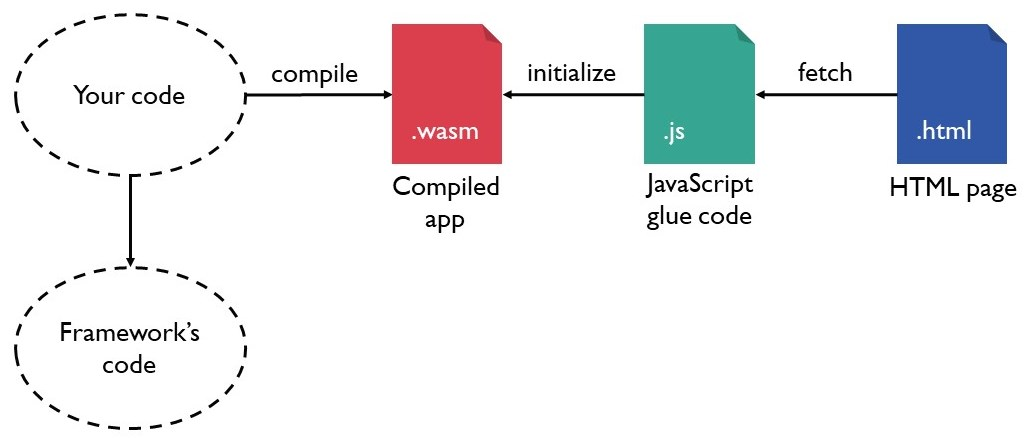
\includegraphics[width=0.95\linewidth]{img/wasm.jpg}
    \caption{\footnotesize Workflow pro WebAssembly \newline Zdroj: {M}{I}{H}{A}{Y}{L}{O}{V}, {B}oyan. {H}ow {W}eb{A}ssembly influences existing {J}ava{S}cript frameworks. {B}oyan {M}ihaylov / {S}oftware architect, web enthusiast, improviser [online]. {A}ugust 26, 2018 [cit. 2022-4-25]. {D}ostupné z: {\tiny \url{https://boyan.io/how-webassembly-influences-existing-javascript-frameworks}}}
    \label{fig:my_label}
\end{figure}
\end{frame}


\defverbatim[colored]\lstIII{
\begin{lstlisting}[language=Rust,basicstyle=\ttfamily,keywordstyle=\color{red}]
#[cfg(not(target_arch = "wasm32"))]
use std::time::{SystemTime, UNIX_EPOCH};
#[cfg(target_arch = "wasm32")]
use wasm_timer::{SystemTime, UNIX_EPOCH};
\end{lstlisting}
}

\defverbatim[colored]\lstIIII{
\begin{lstlisting}[language=Rust,basicstyle=\ttfamily,keywordstyle=\color{red}]
#[cfg(not(target_arch = "wasm32"))]
pub fn nepotrebna_funkce(factor: u8) {
    /* ... */
}
\end{lstlisting}
}

\begin{frame}{Podmíněná kompilace pro WebAssembly}
\lstIII \pause \lstIIII
\end{frame}

\defverbatim[colored]\lsta{
\begin{lstlisting}[language=Rust,basicstyle=\ttfamily,keywordstyle=\color{red}]
#[cfg(target_arch = "wasm32")]
#[wasm_bindgen]
pub fn main_web(canvas_id: &str) {
    /* ... */
}
\end{lstlisting}
}

\defverbatim[colored]\lstba{
\begin{lstlisting}[language=Bash,basicstyle=\ttfamily,keywordstyle=\color{red}]
wasm-bindgen gol.wasm
\end{lstlisting}
}

\defverbatim[colored]\lstbb{
\begin{lstlisting}[language=HTML,basicstyle=\ttfamily,keywordstyle=\color{red}]
<canvas id="app"></canvas>
<script src="gol.js"></script>
<script>
    wasm_bindgen("./gol_bg.wasm")
        .then(on_wasm_loaded)
        .catch(console.error);
    
    function on_wasm_loaded() {
        wasm_bindgen.main_web("app");
    }
</script>
\end{lstlisting}
}

\begin{frame}{WebAssembly v Rustu}{Implementace dosažitelných funkcí}
\lstba \pause \lstbb
\end{frame}

\begin{frame}{Vytvořená aplikace}{Conwayova Hra života s GUI, portovaná do rozhraní webového prohlížeče}
\begin{figure}[htpb]
    \centering
    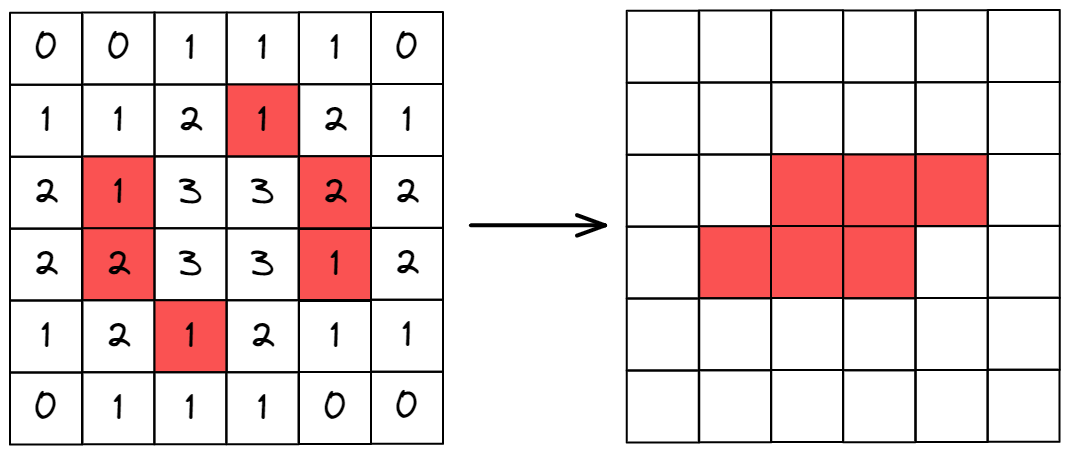
\includegraphics[width=\linewidth]{img/conway.png}
\end{figure}
\end{frame}

\begin{frame}{}{}
\begin{figure}[htpb]
    [demonstrace desktop + WebAssembly aplikace]
\end{figure}
\end{frame}

\end{document}